\section{Lasershow}
Program lasershow se~stará o~vykreslování obrazu podle příkazů od~frontendových programů, patří tedy mezi backendové programy.

Je psán v~kompilovanem jazyce C++, jeho běh je~tedy rychlejší, než kdyby byl~využit interpretovaný jazyk.
Interpretované jazyky bývají pomalejší, protože interpreter musí kód překládat za~běhu a~tím oddaluje jeho exekuci~\cite{interpret}.
To je~důležité, protože při vykreslování každá ztracená milisekunda může znamenat nežádoucí efekty. I~při vykreslování jednoduchých obrazců zaseknutí paprsku na~jednom místě způsobí přesvětlený bod.

\subsection{Inspirace open-source}
Program byl~inspirován projektem rpi-lasershow~\cite{rpi-lasershow}. Zmíněný projekt posloužil jako předloha struktury promítání, ovšem všechny jeho části byly přepsány, aby~umožňovaly pokročilé funkce výsledného programu lasershow.

Velkou výhodou oproti zmíněnému programu je~možnost s~programem interagovat.
Původní program lasershow totiž po~spuštění jednoduše přečetl soubor, který mu~byl~předán jako argument, a~začal ho~promítat. Promítání bylo možné přerušit pouze zastavením programu.

\subsection{Funkce programu}
Díky nově implementovaným interakcím je~možné ve~frontendových programech ovládat mnoho aspektů projekce popsaných v~následujících kapitolách. Program lasershow je~schopen přijímat příkazy od~frontendových programů a~reagovat na~ně i~při vykreslování probíhající projekce. Program také všechny informace o~probíhající projekci a~nadcházejících projekcích posíla frontendovým programům, aby~je~zobrazily uživateli.

\subsubsection{Spouštění projekcí}
Je možné vybrat soubor k~projekci, vytvářet frontu projekcí, které se~spustí za~sebou, nastavit opakování jedné projekce, nebo celé fronty a~také se~posouvat v~časové ose~projekce (tzn. například skočit na~200. snímek právě probíhající projekce).

\subsubsection{Nastavení projekce}
Nastavením projekcí jsou myšleny:
\begin{itemize}
\item Ovládání jasu jednotlivých laserových diod.
\item Deformace obrazu pro~kompenzaci úhlu vůči plátnu.
\item Změna velikosti a~posun projekce. 
\item Rychlosti vykreslování -- ta~je~úrčena časem, kdy~projektor čeká mezi vykreslením jednotlivých bodů.
\item Rychlost časového průběhu projekce -- ta~je~úrčena časem, po~kterém projektor přeskočí na~další snímek projekce.
\item Vykreslování vždy úplných snímků -- program může buď snímek přerušit ve~chvíli, kdy~je~překročen čas úrčený pro~snímek, nebo může po~uplynutí tohoto času vždy dokreslit body snímku, které nestihl vykreslit.
\item Časově přesného snímkování -- při zapnutí časově přesného snímkování program vždy vybere k~projekci snímek, který by~se~měl v~danou chvíli promítat podle času, který uplynul od~začátku projekce místo jednoduchého pokračování ve~frontě snímků.
\end{itemize}


\subsection{Využité knihovny}
\subsubsection{cppzmq}\label{sec:ls_cppzmq}
Knihovna cppzmq~\cite{cppzmq} je~knihovna zprostředkující sockety ZeroMQ v~jazyce C++. Využití této knihovny je~vidět v~ukázce kódu~\ref{list:zmq_s_cpp}.
\begin{code}
  \captionof{listing}{\label{list:zmq_s_cpp} Využití knihovny cppzmq v~programu lasershow}
  \inputminted[frame=lines,fontsize=\footnotesize{}, linenos, breaklines]{cpp}{code_examples/zmq_server.cpp}
\end{code}

% Mezi nejdůležitější mnou využité funkce této knihovny patří:
% \begin{itemize}
%   \item \mintinline{cpp}{zmq::context_t::context_t(int io_threads)} --- Kontruktor třídy \mintinline{cpp}{zmq::context_t}; Tato třída je~nutná k~vytvoření socketů.
%   \item \mintinline{cpp}{zmq::socket_t::socket_t(context_t &context, int~type)} --- Kontruktor třídy \mintinline{cpp}{zmq::socket_t}; Ta~je~nutná registraci socketů, příjmání zpráv i~odesílání zpráv. Argument type určuje chování socketu. Já v~jeho místě využívám hodnotu \mintinline{cpp}{zmq::socket_type::pub} pro~odesílání do~socketu a~\mintinline{cpp}{zmq::socket_type::sub} pro~příjmání zpráv socketem.
%   \item \mintinline{cpp}{void zmq::socket_t::bind(const char *endpoint)} --- Funkce, která k~socketu zaregistruje určitou adresu. V~mém kódu vypadá například takto \mintinline{cpp}{command_receiver.bind("tcp://*:5557");}, kdy~\mintinline{cpp}{command_receiver} je~třída \mintinline{cpp}{zmq::socket_t} a~5557 je~port, na~kterém bude socket naslouchat.
%   \item \mintinline{cpp}{void zmq::socket_t::set(sockopt::array_option<Opt, NullTerm>, const std::string &buf)} --- Funkce nastavující vlastnost socketu. Ta~je~v mém kódu využita následovně k~nastavení příjmání všech zpráv v~socketu, který příjmá zprávy. \mintinline{cpp}{command_receiver.set(zmq::sockopt::subscribe, "");}
%   \item \mintinline{cpp}{bool zmq::socket_t::recv(message_t *msg, int~flags = 0)} --- Funkce se~pokusí příjmout zprávu ze~socketu, jehož třídě náleží, a~uložit ji~do~objektu \mintinline{cpp}{zmq::message_t}, na~nějž jí byl~předán pointer v~prvním argumentu. Při použití této funkce v~argumentu \mintinline{cpp}{flags} používám buď hodnotu \mintinline{cpp}{zmq::recv_flags::none}, nebo hodnotu \mintinline{cpp}{zmq::recv_flags_::dontwait}.
% V~prvním případě se~exekuce při zavolání této funkce zastaví do~chvíle, kdy~přijde socketem zpráva. V~druhém případě exekuce pokračuje i~přesto, že nebyla přijmuta žádná zpráva. Funkce vrací hodnotu true jestliže zpráva byla úspěšně přijata a~uložena. Jindy vrací hodnotu flase.
%   \item \mintinline{cpp}{bool zmq::socket_t::send(message_t &msg, int~flags = 0)} --- Funkce se~pokusí poslat do~socketu, jehož třídě náleží, zprávu z~prvního argumentu. V~druhém argumentu vždy používám hodnotu \mintinline{cpp}{zmq::send_flags::none}.
% \end{itemize}

\subsubsection{ADCDACPi}
Knihovna ADCDACPi~\cite{ADCDACPi} zjednodušuje komunikaci s~D/A převodníkem mcp4822, využitém v~generátoru signálu pro~galvanometry, viz~kapitola~\ref{sec:ilda-signal-gen}, přes rozhraní SPI. Její použití je~vidět na~ukázce kódu~\ref{list:adcdac}.
\begin{code}
  \captionof{listing}{\label{list:adcdac} Využití knihovny ADCDACPi v~programu lasershow}
  \inputminted[frame=lines,fontsize=\footnotesize{}, linenos, breaklines]{cpp}{code_examples/adcdac.cpp}
\end{code}

% Mezi nejdůležitější mnou využité funkce této knihovny patří:
% \begin{itemize}
%   \item \mintinline{cpp}{int ADCDACPi::open_dac()} --- Tuto funkci je~potřeba zavolat před použitím D/A převodníku. Inicializuje SPI~komunikaci s~D/A převodníkem. Vrací 1, pokud je~inicializace úspěšná a~0, pokud neúspěšná. komunikace musí být inicializovaná, aby~bylo možné D/A převodníku posílat instrukce.
%   \item \mintinline{cpp}{void ADCDACPi::set_dac_raw(uint16_t raw, int~channel)} --- Funkce, která zašle D/A převodníku insrtukci, aby~nastavil na~kanálu uvedeném v~argumentu \mintinline{cpp}{channel} napětí odpovídající $\frac{raw}{4096} \times V_{ref}$, kdy~$raw$ je~parametr předaný funkci, $4096$ je~rozlišení D/A převodníku a~$V_{ref}$ je~referenční napětí připojené k~D/A převodníku.
%   \item \mintinline{cpp}{void ADCDACPi::close_dac()} --- Funkce deinicializuje SPI~komunikaci s~D/A převodníkem. Měla by~být zavolána před ukončením programu.
% \end{itemize}
\subsubsection{pigpio}\label{sec:ls_pigpio}
Knihovna pigpio~\cite{pigpio} umožňuje ovládání GPIO pinů Raspberry Pi. Je~využita k~posílání PWM~signálu do~laserového modulu. Příklad využití PWM~funkcí knihovny je~vidět v~ukázce kódu~\ref{list:pigpio_pwm}.

\begin{code}
  \captionof{listing}{\label{list:pigpio_pwm} Využití PWM~funkcí knihovny pigpio v~programu lasershow}
  \inputminted[frame=lines,fontsize=\footnotesize{}, linenos, breaklines]{cpp}{code_examples/pigpio_pwm.cpp}
\end{code}

% Mezi nejdůležitější mnou využité funkce této knihovny patří:
% \begin{itemize}
%   \item \mintinline{cpp}{int gpioInitialise()} --- Funkce, která inicializuje knihovnu pigpio. Musí být zavolána před použitím dalších funkcí.
%   \item \mintinline{cpp}{int gpioSetMode(unsigned gpio, unsigned mode)} --- Funkce, která pro~GPIO pin~z argumentu \mintinline{cpp}{gpio} nastaví mód z~argumentu \mintinline{cpp}{mode}. Jako argument \mintinline{cpp}{mode} používám hodnotu \mintinline{cpp}{PI_INPUT}, která pin~zaregistruje pro~vstup, a~hodnotu \mintinline{cpp}{PI_OUTPUT}, která pin~zaregistruje pro~výstup.
%   \item \mintinline{cpp}{int gpioSetPullUpDown(unsigned gpio, unsigned pud)} --- Funkce připojí na~pin~\mintinline{cpp}{gpio} pull-up nebo pull-down rezistor podle argumentu \mintinline{cpp}{pud}.
%   \item \mintinline{cpp}{int gpioSetPWMfrequency(unsigned user_gpio, unsigned frequency)} --- Funkce, která na~pinu \mintinline{cpp}{user_gpio} nastaví frekvency PWM~pulzů na~parametr \mintinline{cpp}{frequency} v~Hz.
%   \item \mintinline{cpp}{int gpioPWM(unsigned user_gpio, unsigned dutycycle)} --- Tato funkce na~pinu \mintinline{cpp}{user_gpio} nastaví střídu PWM, pokud je~pin~zaregistrován pro~výstup.
%   \item \mintinline{cpp}{int gpioWrite(unsigned gpio, unsigned level)} --- Pokud je~pin~\mintinline{cpp}{gpio} Funkce nastaví něm výstup dle~parametru \mintinline{cpp}{level}. Ten~může mít hodnoty \mintinline{cpp}{1}, nebo \mintinline{cpp}{0}
%   \item \mintinline{cpp}{uint32_t gpioDelay(uint32_t micros)} --- Funkce pozastaví exekuci programu na~\mintinline{cpp}{micros} mikrosekund.
% \end{itemize}

\subsection{Struktura programu}
Struktura programu je~vidět ve~zjedonušeném obrázku~\ref{fig:lasershow-flowchart} a~je~popsána na~dalších stránkách.

% \newgeometry{top=0mm, bottom=0mm, left=0mm, right=0mm}

\begin{figure}[H]
  \centering
  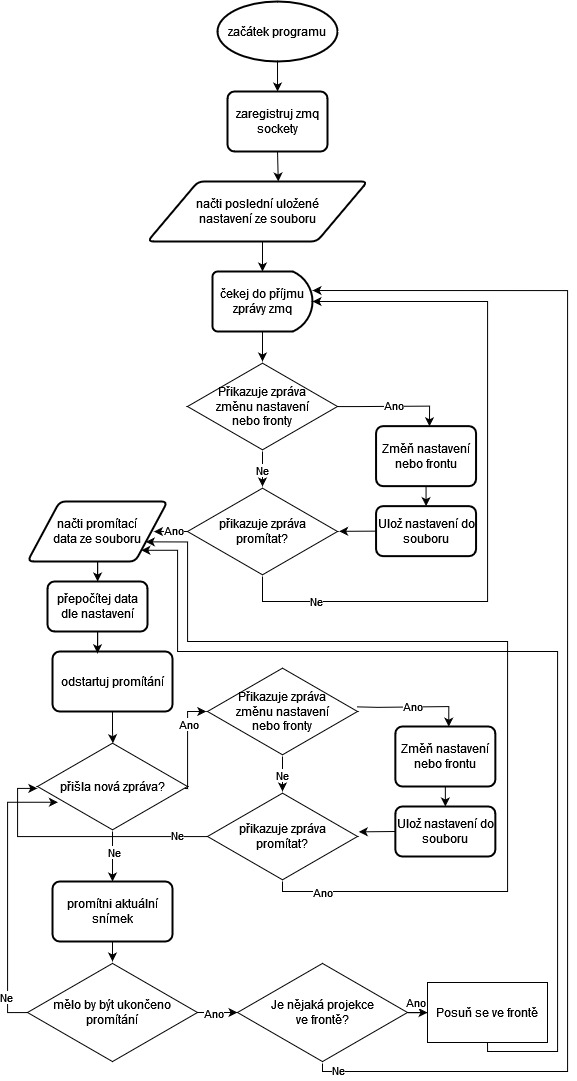
\includegraphics[width=\textwidth{}, trim=0 600 0 0, clip]{img/lasershow_flowchart.jpg}
  \caption{\label{fig:lasershow-flowchart} Diagram programu lasershow; Pokračuje na~další stránce.}
\end{figure}
\clearpage
\begin{figure}[H]
  \centering
  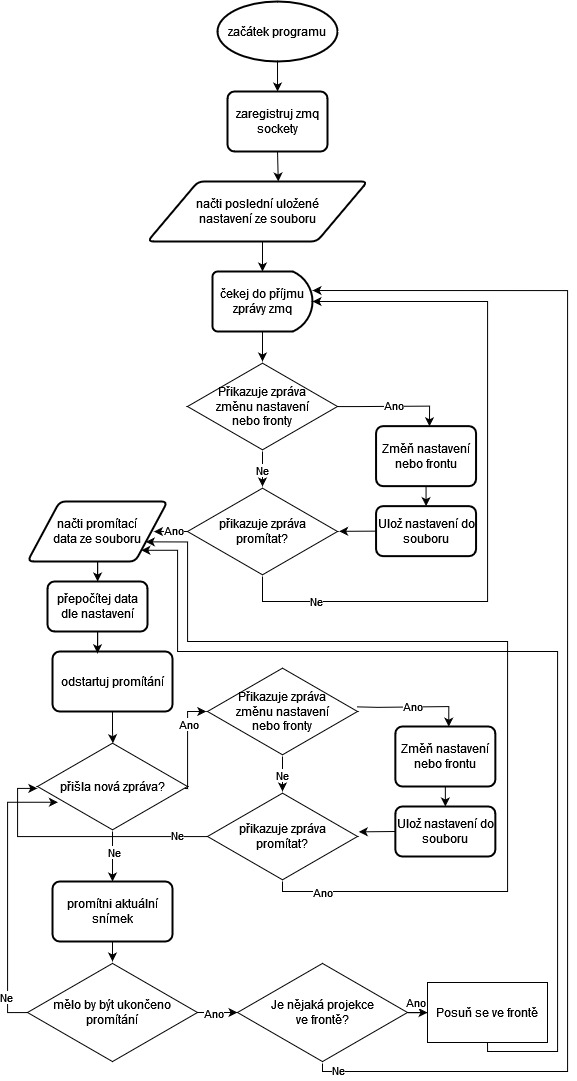
\includegraphics[width=\textwidth{}, trim=0 0 0 350, clip]{img/lasershow_flowchart.jpg}\clearpage
\end{figure}


\restoregeometry

Tento program pomocí knihovny ZeroMQ zaregistruje svůj vstupní a~výstupní socket a~přihlásí se~na~tom~vstupním k~odběru zpráv.

Následně načte konfigurační soubor lasershow.cfg, který obsahuje uložené nastavení z~posledního běhu programu a~čeká na~příchozí zprávy.

Jakmile přijde zpráva, přečte ji. Pokud je~požadována změna nastavení, okamžitě ji~provede, aktuální nastavení si~uloží do~souboru lasershow.cfg a~přepočítá informace o~promítaném obrazu, je-li to~nutné (Například, změní-li se~nastavení trapezoid-horizontal, přepočítá souřadnice vykreslovaných bodů).
Jestliže je~požadováno vykreslení obrazu ze~souboru, načte soubor a~začne obraz vykreslovat.
Přitom průběžně posílá informace o~stavu vykreslování do~výstupního socketu.
I~při vykreslování obrazu tento program zpracovává zprávy a~pokyny ze~vstupního socketu.

\section{wifi\_manager}

Program wifi\_manager se~přímo nepodílí ani~na~projekci, ani~na~interakci s~uživatelem. Mění totiž WiFi připojení, pokud uživatel prostřednictvím nějakého frontendového programu tuto změnu vyžádá.

Program wifi\_manager je~napsaný v~jazyce JavaScript s~využitím runtime Node.js.

\subsection{Funkce programu}
Program umožňuje uživateli měnit nastavení WiFi připojení Raspberry Pi. Nastavením WiFi připojení jsou myšleny tři stavy.
Prvním stavem je~\uv{WiFi}, kdy~Raspberry Pi~vyhledává v~okolí známé sítě, ke~kterým by~se~mohlo připojit.
Druhým stavem \uv{Hotspot}, v~tomto stavu Raspberry Pi~vysílá vlastní WiFi síť, ve~které se~stalo přístupovým bodem.
A třetím stavem je~\uv{WiFi připojení vypnuto}, kdy~je~WiFi anténa Raspberry Pi~neaktivní.

Program má také svůj konfiguranční soubor, kam~si, podobně jako lasershow, ukládá aktuální nastavení, aby~si~ho~\uv{pamatoval} i~po~restartu systému.

\subsubsection{Služby obsluhující WiFi připojení}
Spuštění přístupopvého bodu na~Raspberry Pi~totiž není tak~jednoduché, je~při něm potřeba změnit nastavení dvou služeb umožňujících provoz hotspotu a~restartovat je. Tyto služby jsou hostapd a~dnsmasq.
Hostapd je~služba umožňující využití Raspberry Pi~jako přístupového bodu. Spravuje například ověření totožnosti připojovaných zařízení~\cite{hostapd}. Dnsmasq je~služba, která umožňuje přiřazovat připojeným zařízením IP~adresy~\cite{dnsmasq}.

Naopak při přechodu do~normálního \uv{WiFi} módu je~potřeba tyto služby deaktivovat a~spustit službu dhcpcd. Ta~se~chová jako klient pro~komunikaci s~přístupovým bodem protokolem DHCP~\cite{dhcpcd}. Umožňuje tedy přístupovému bodu dynamicky přiřadit Raspberry Pi~lokální IP~adresu.

WiFi manager tedy existuje, aby~sjednotil toto nastavování do~jednoho programu. Bylo by~totiž nepraktické, kdyby musely stejnou akci provádět ostatní programy, které jsou psané v~různých jazycích.

Ke spouštění těchto služeb je~využíván manažer systému a~služeb systemd. Ten~je~součástí mnoha systémů založených na~kernelu Linux. Při každém zapnutí systému je~spuštěn jako první program a~stará se~o~spuštění všech ostatních programů.~\cite{systemd}

\subsection{Využité knihovny}
\subsubsection{child\_process}
V programu je~využita funkce \mintinline{bash}{execSync(command[, options])} z~knihovny \mintinline{bash}{child_process} pro~spouštění systémových příkazů. To~je~potřeba pro~zastavení zmíněných systémových služeb a~k umožnění změn v~jejich nastavení.

Tyto služby jsou zastavovány a~spouštěny pomocí softwaru systemd a~jeho nástroje v~příkazovém řádku zvaném \mintinline{bash}{systemctl}.
V mém kódu tudíž používám funkci \mintinline{js}{execSync} k~zastavení služeb hostapd a~dnsmasq následovně \mintinline{js}{execSync("sudo systemctl disable hostapd dnsmasq")}.

\subsubsection{Zeromq.js}
Dále je~v~programu využita knihovna zeromq.js~\cite{zeromqjs} pro~komunikaci s~ostatními programy. Jak~je~použita, je~vidět v~ukázce kódu~\ref{list:zmq_s_js}.

\begin{code}
  \captionof{listing}{\label{list:zmq_s_js} Využití knihovny zeromq.js v~programu wifi\_manager}
  \inputminted[frame=lines,fontsize=\footnotesize{}, linenos, breaklines]{js}{code_examples/zmq_server.js}
\end{code}

\subsection{Struktura programu}

Registruje pro~sebe dva~sockety stejně jako lasershow, jedním přijímá příkazy týkající se~nastavení WiFi a~druhým odesílá zpětnou vazbu o~aktuálním WiFi připojení. Zároveň registruje callback funkci, která se~spustí při přijetí zprávy vstupním socketem.

Když příjme příkaz pro~změnu připojení, zkontroluje, jestli připojení tomuto příkazu už nevyhovuje. Pokud mu~nevyhovuje, nejdříve si~zapíše do~svého konfiguračního souboru požadovaný stav wifi připojení. Následně zastaví služby hostapd, dnsmasq a~dhcpcd, změní jim~nastavení dle~konfiguračních souborů předem uložených ve~své složce a~opět některé z~nich spustí podle toho, jakého stavu WiFi připojení se~snaží dosáhout.
Pro \uv{Hotspot} stav je~potřeba, aby~byly spuštěny služby hostapd, dnsmasq a~dhcpcd, pro~normální \uv{WiFi} stav je~potřeba spuštěná pouze služba dhcpcd.

Může také příjmat příkazy, které pouze požadují hlášení o~nastavení WiFi připojení a~nechtějí toto nastavení nějak měnit. Při přijetí takového příkazu wifi\_manager přečte svůj konfigurační soubor a~pošle do~svého výstupního socketu zprávu odpovídající aktuálnímu nastavení.
